% !TeX program = pdfLaTeX
\documentclass[smallextended]{svjour3}       % onecolumn (second format)
%\documentclass[twocolumn]{svjour3}          % twocolumn
%
\smartqed  % flush right qed marks, e.g. at end of proof
%
\usepackage{amsmath}
\usepackage{graphicx}
\usepackage[utf8]{inputenc}

\usepackage[hyphens]{url} % not crucial - just used below for the URL
\usepackage{hyperref}

%
% \usepackage{mathptmx}      % use Times fonts if available on your TeX system
%
% insert here the call for the packages your document requires
%\usepackage{latexsym}
% etc.
%
% please place your own definitions here and don't use \def but
% \newcommand{}{}
%
% Insert the name of "your journal" with
% \journalname{myjournal}
%

%% load any required packages here



% tightlist command for lists without linebreak
\providecommand{\tightlist}{%
  \setlength{\itemsep}{0pt}\setlength{\parskip}{0pt}}



\usepackage{booktabs}
\usepackage{longtable}
\usepackage{array}
\usepackage{multirow}
\usepackage{wrapfig}
\usepackage{float}
\usepackage{colortbl}
\usepackage{pdflscape}
\usepackage{tabu}
\usepackage{threeparttable}
\usepackage{threeparttablex}
\usepackage[normalem]{ulem}
\usepackage{makecell}
\usepackage{xcolor}
\begin{document}


\title{Transfer of Learned Opponent Models in Zero Sum Games \thanks{The authors have no conflicts of interest to declare that are relevant
to the content of this article. This work was supported by the UK
Engineering and Physical Sciences Research Council under grant
EP/S515255/1.} }



\author{  Ismail Guennouni \and  Maarten Speekenbrink \and  }


\institute{
        Ismail Guennouni \at
     Department of Experimental Psychology, University College London, 26
 Bedford Way, London WC1H 0AP, United Kingdom \\
     \email{\href{mailto:i.guennouni.17@ucl.ac.uk}{\nolinkurl{i.guennouni.17@ucl.ac.uk}}}  %  \\
%             \emph{Present address:} of F. Author  %  if needed
    \and
        Maarten Speekenbrink \at
     Department of Experimental Psychology, University College London, 26
 Bedford Way, London WC1H 0AP, United Kingdom \\
     \email{\href{mailto:m.speekenbrink@ucl.ac.uk}{\nolinkurl{m.speekenbrink@ucl.ac.uk}}}  %  \\
%             \emph{Present address:} of F. Author  %  if needed
    \and
    }

\date{Received: date / Accepted: date}
% The correct dates will be entered by the editor


\maketitle

\begin{abstract}
Human learning transfer abilities take advantage of important cognitive
building blocks such as an abstract representation of concepts
underlying tasks and causal models of the environment. One way to build
abstract representations of the environment when the task involves
interactions with others is to build a model of the opponent that may
inform what actions they are likely to take next. In this study, we
explore opponent modelling and its transfer in games where human agents
play against computer agents with human-like limited degrees of iterated
reasoning. In two experiments, we find that participants deviate from
Nash equilibrium play and learn to adapt to their opponent's strategy to
exploit it. Moreover, we show that participants transfer their learning
to new games. Computational modelling shows that players start each game
with a model-based learning strategy that facilitates between-game
transfer of their opponent's strategy, but then switch to behaviour that
is consistent with a model-free learning strategy in the latter stages
of the interaction.
\\
\keywords{
        Learning Transfer \and
        Opponent Modelling \and
        Hidden Markov Models \and
        Bayesian Cognitive Hierarchy \and
    }


\end{abstract}


\def\spacingset#1{\renewcommand{\baselinestretch}%
{#1}\small\normalsize} \spacingset{1}


\hypertarget{introduction}{%
\section{Introduction}\label{introduction}}

Being able to transfer previously acquired knowledge to a new domain is
one of the hallmarks of human intelligence. This ability relies on
important cognitive building blocks, such as an abstract representation
of concepts underlying tasks (Lake et al. 2017). One way to form these
representations when the task involves interactions with others, is to
build a model of the person we are interacting with that offers
predictions of the actions they are likely to take next. There is
evidence that people learn such models of their opponents when playing
repeated economic games (Stahl and Wilson 1995). A model of the opponent
can help increase performance in a particular game, but learning more
general characteristics of an opponent may also help increase
performance in other games. In this paper, we are specifically
interested in the latter: How do people build and use models of their
opponent to facilitate learning transfer?

Repeated games, in which players interact repeatedly with the same
opponent and have the ability to learn about their opponent's strategies
and preferences (Mertens 1990) are particularly useful to address this
question. The early literature on learning transfer in repeated games
has mostly focused on the proportion of people who play normatively
optimal (e.g.~Nash equilibrium play) or use salient (e.g.~risk
dominance) actions in later games, having had experience with a similar
game environment previously (Ho, Camerer, and Weigelt 1998; Knez and
Camerer 2000). As is well-known, a Nash equilibrium means that all
players in a game act such that no-one can unilaterally improve their
performance by deviating from their strategy. When playing against an
opponent with a Nash-optimal strategy, you can do no better than play
according to the Nash-equilibrium strategy as well. However, when faced
with a player who deviates from the Nash-optimal strategy, you may be
able to exploit this and also deviate from this strategy, increasing
your performance beyond what is expected at Nash equilibrium. Of course,
this comes with a risk, as your own deviation from Nash-optimal play may
leave you open to similar exploitation.

Studies that focused on whether people can learn to exploit deviations
from Nash-equilibrium play have mostly looked at the ability of players
to detect and exploit contingencies in their opponent's actions (Dyson
et al. 2016; Spiliopoulos 2013; Shachat and Swarthout 2004). These
studies used computer opponents that don't adapt their strategy to their
human opponent, mostly consisting of playing each action with a fixed
probability (a mixed strategy) or using a pre-determined sequence.
Findings show that humans are capable of adapting to
non-Nash-equilibrium play and detect patterns in an opponent's history
of play. However, the use of mixed strategies may have limited people's
ability to form accurate opponent models.

The game of Rock-Paper-Scissors (RPS) has emerged as a central paradigm
to test sequential adversarial reasoning in repeated interactions.
Beyond action frequencies, Dyson (2019) identifies cycle-based and
outcome-based dependencies as important strategies in repeated RPS
games. A positive cycle is when a player chooses in trial \(t+1\) an
action that would have beaten the action in trial \(t\) (e.g., playing
Paper after Rock), while a negative cycle goes in the opposite direction
by choosing an action in trial \(t+1\) that would have been beaten by
the action on trial \(t\) (e.g., playing Scissors after Rock). These
cycle-based strategies can be based on the opponent's or a player's own
past choices. For example, Eyler et al. (2009) show that players have a
tendency to repeat their previous-round actions. Brockbank and Vul
(2021) defined a hierarchy of strategies based on previous actions (base
rate of choices) as well as cycle transitions (base rate of positive and
negative cycles). Using data on dyads playing 300 rounds of RPS against
the same opponent, they show that exploitation of non-random play
leverages simple regularities between a player's next action and their
own previous action, and between a player's next action and their
opponent's previous action, while more complex regularities remain
unexploited. Outcome based dependencies are another common basis for RPS
strategies. The idea is to change the likelihood of future actions based
on the outcome (win, loss, or tie) of the previous round. Heuristics
such as win-stay/lose-shift are an example of such outcome dependencies.
Players can also combine outcome and cycle based strategies, choosing to
cycle in a positive or negative direction depending on whether the
previous round was won or lost (Wang, Xu, and Zhou 2014; Xu, Zhou, and
Wang 2013).

Another way to frame these strategies is in terms of iterative
reasoning. People may think of their opponents as applying a limited
number of recursive steps to determine their next action. The type of
reasoning we refer to takes the form of ``I believe that you believe
that I believe \ldots{}''. For example, if I believe that you believe I
will play Rock (perhaps because I played Rock in the previous round),
then I would expect you to play Paper, as this beats my Rock. I would
therefore choose to play Scissors, as this beats your Paper. This
results in a self-directed negative cycle strategy (playing the action
that beats ones previous action), but it is the result of applying one
level of recursive reasoning (player A believes player B believes A will
repeat their last action, and A best responds to player B's best
response to this belief).

Strategies based on iterative reasoning can explain non-equilibrium play
in a range of games (Camerer 2003), such as the \(p\)-beauty contest
game (Nagel 1995), dominance solvable games (Camerer, Ho, and Chong
2004), and various standard normal form games (Costa-Gomes, Crawford,
and Broseta 2001). They also underlie successful models in behavioural
economics, such as Level-\(k\) and Cognitive Hierarchy models (Camerer,
Ho, and Chong 2004), which posit that people assume their opponent
applies a limited level of iterative reasoning, taking actions that are
best responses to those of their (modelled) opponent. In Level-\(k\)
theory, a level-0 player uses a fixed strategy without explicitly
considering the strategy of their opponent. A level-1 player assumes
their opponent is a level-0 player, and chooses actions to best respond
to the strategy of their opponent, without considering what their
opponent might believe that they will play. A level-2 player, on the
other hand, takes their opponent's belief about their actions into
account, assuming they face a level-1 player, and choosing actions to
best respond to the actions of that player. Cognitive Hierarchy theory
is based on similar principles, but rather than assuming an opponent
always adopts a particular level-\(k\) strategy, they are assumed to
adopt each of the level-\(k\) strategies with a particular probability
(i.e., the opponent's strategy is a mixture over pure level-\(k\)
strategies).

Batzilis et al. (2019) analysed data from a million online RPS games and
found that players strategically used information on their opponents'
previous play. While the majority of play (74\%) is consistent with a
level-0 strategy, a significant proportion is consistent with either a
level-1 (19\%) or level-2 strategy (7\%). As noted above, iterative
reasoning results in specific action contingencies which correspond to
particular action, outcome, and cycle based strategies. Prior research
analysing behaviour in terms of these latter strategies has not
explicitly related these to levels of iterative reasoning. That
particular patterns are observed more frequently, and are exploited more
readily (Brockbank and Vul 2021), may be due to people adopting specific
forms of iterative reasoning. For example, using a sequential move game,
Hedden and Zhang (2002) found that people initially adopt a level-1
strategy, thus assuming their opponent to adopt a level-0 strategy, but
can learn over time to adopt a level-2 strategy if their opponent
consistently uses a level-1 strategy. In a different version of this
sequential move game, Goodie, Doshi, and Young (2012) found that
participants initially adopt a level-2 strategy, but over time can learn
to adopt a level-1 strategy if the opponent consistently uses a level-0
strategy. To what extent these results generalise to simultaneous move
games such as RPS is unclear. Zhang, Moisan, and Gonzalez (2021) found
that people can learn to beat computer opponents adopting a win-stay
lose-change or win-change lose-stay strategy, which are both level-0
strategies.

There are three main ways in which you can learn to exploit a
level-\(k\) opponent. One way is to explicitly learn the depth of their
iterative reasoning, such as that the opponent's actions are based on a
level-2 strategy. The second way is to learn the contingencies between
previous round play and an opponent's next action (e.g., that your
opponent is likely to play Scissors if your previous action was Paper).
Rather than learning to predict an opponent's next actions, and then
deciding upon the best counter-move, a third strategy is to directly
learn rewarding actions. Unlike learning contingencies between actions,
or which current action is most rewarding, learning the depth of
iterative reasoning allows for generalisation to other games with
different actions. This can then provide an early advantage, allowing
one to exploit the opponent's strategy before you have played long
enough to reliably establish contingencies within a game. In what we
call the Bayesian Cognitive Hierarchy model, we propose that people use
Bayesian inference to determine the depth of iterative reasoning of
their opponent, and use this to predict their opponent's actions and
determine the best response to this. We contrast this to a Reinforcement
Learning model, which learns which actions are most rewarding given
previous round play, by learning state-action values (the expected
reward from taking an action in a given state). The Experience Weighted
Attraction (EWA) model (Ho, Camerer, and Chong 2007), popular in
behavioral game theory, includes an additional mechanism to learn about
the consequences of actions that were not actually taken.

As both RL and EWA models learn values for actions in states (here, we
define the state as the previous play), they don't allow for
generalization to new games with different actions, as there is no
immediate way in which to map a set of actions in one game to a set of
actions in another. For example, consider the game of Fire-Water-Grass
(FWG), where water beats fire, grass beats water, and fire beats grass.
This game is structurally the same as RPS. However, if you have learned
in RPS to play Rock after a previous play of Paper, there is no direct
way to transfer this to knowing that Fire is a rewarding move after
previously having played Water. Learning about the new actions in FWG
requires experience with the FWG game. This is in contrast to learning
the level of iterative reasoning of the opponent. If you know they
expect you to repeat your previous action and choose their action to
beat this, then you can infer that they will play Grass after your
previous choice of Water, even if you have never played FWG before.
Whilst providing a way to transfer knowledge about an opponent to new
games, iterative reasoning is likely to be more cognitively demanding
than learning action contingencies. Once sufficient experience has been
gained within a game, iterative reasoning may no longer provide an
advantage over simpler reinforcement learning. Therefore, it might be
more efficient to use an RL strategy in the later stages of a game. In
our modelling, we will allow for such switching between strategies
during games.

In the present study, we let humans repeatedly face computer agents
endowed with a limited ability for iterative reasoning based on
previous-round play. As in previous studies discussed above, we use
computer opponents to enable precise experimental control over the
strategies used and the transfer of depth of iterative reasoning between
games. We aim to assess whether (1) human players adapt their strategy
to exploit this limited reasoning of their opponent, and (2) whether
they are able to generalize a learned opponent model to other games. In
two experiments, participants repeatedly face the same opponent
(Experiment 1) or two different opponents (Experiment 2) in three
consecutive games: the well-known Rock-Paper-Scissors game, the
structurally similar Fire-Water-Grass game, and a less similar Numbers
(Experiment 1) or Shootout (Experiment 2) game. To foreshadow our
results, we find evidence that participants transfer the learned
strategy of their opponent to new games, providing them with an early
advantage before gaining enough experience within a game to enable
learning contingencies between previous and winning actions.
Computational modelling shows that participants, when first encountering
an opponent in a new game, employ Bayesian inference about the level of
iterative reasoning of their opponent to predict their actions and
determine the best response. However, in later rounds of the games, they
switch to a cognitively less demanding reinforcement learning strategy.

\hypertarget{experiment-1}{%
\section{Experiment 1}\label{experiment-1}}

In the first experiment, we aim to test learning transfer by making
participants face the same computer opponent with a limited level of
iterative reasoning in three sequential games that vary in similarity.
If participants are able to learn the limitations of their opponent's
iterative reasoning and generalize this to new games, their performance
in (the early stages of) later games should be higher than expected if
they were to completely learn a new strategy in each game.

\hypertarget{methods}{%
\subsection{Methods}\label{methods}}

\hypertarget{participants-and-design}{%
\subsubsection{Participants and Design}\label{participants-and-design}}

A total of 52 (28 female, 24 male) participants were recruited on the
Prolific Academic platform. The mean age of participants was 31.2 years.
Participants were paid a fixed fee of £2.5 plus a bonus dependent on
their performance (£1.06 on average). The experiment had a 2 (computer
opponent: level-1 or level-2) by 3 (games: rock-paper-scissors,
fire-water-grass, numbers) design, with repeated measures on the second
factor. Participants were randomly assigned to one of the two levels of
the first factor.

\hypertarget{tasks}{%
\subsubsection{Tasks}\label{tasks}}

Participants played three games against their computer opponent:
Rock-Paper-Scissors (RPS), Fire-Water-Grass (FWG), and the Numbers game.
RPS is a 3x3 zero-sum game, with a cyclical hierarchy between the two
player's actions: Rock blunts Scissors, Paper wraps Rock, and Scissors
cut Paper. If one player chooses an action which dominates their
opponent's action, the player wins (receives a reward of 1) and the
other player loses (receives a reward of -1). Otherwise it is a draw and
both players receive a reward of 0. RPS has a unique mixed-strategy Nash
equilibrium, which consists of each player in each round randomly
selecting from the three options with uniform probability.

The FWG game is identical to RPS in all but action labels: Fire burns
Grass, Water extinguishes Fire, and Grass absorbs Water. We use this
game as we are interested in whether learning is transferred to a
fundamentally similar game, where the only difference is in the label of
the possible actions. This should make it relatively easy to generalize
knowledge of the opponent's strategy, provided this knowledge is on a
sufficiently abstract level, such as knowing the opponent is a level-1
or level-2 player. Crucially, learning simple contingencies such as ``If
I played Rock on the previous round, playing Scissors next will likely
result in a win'', is not generalizable to this similar game, as these
contingencies are tied to the labels of the actions.

The Numbers game is a generalization of RPS. In the variant we use, 2
participants concurrently pick a number between 1 and 5. To win in this
game, a participant needs to pick a number exactly 1 higher than the
number chosen by their opponent. For example, if a participant thinks
their opponent will pick 3, they ought to choose 4 to win the round. To
make the strategies cyclical as in RPS, the game stipulates that the
lowest number (1) beats the highest number (5), so if the participant
thinks the opponent will play 5, then the winning choice is to pick 1.
This game has a structure similar to RPS in which every action is
dominated by exactly one other action. All other possible combinations
of choices are considered ties. Similar to RPS and FWG, the
mixed-strategy Nash equilibrium is to randomly choose each action with
equal probability.

The computer opponent was programmed to use either a level-1 or level-2
strategy in all the games. A level-1 player is defined as a player who
best responds to a level-0 player. A level-0 player does not consider
their opponent's beliefs. Here, we assume a level-0 player simply
repeats their previous action. There are other ways to define a level-0
player. For instance, as repeating their action if it resulted in a win
and choosing randomly from the remaining actions otherwise, or choosing
randomly from all actions. As a best response to a uniformly random
action is itself a random action, defining a level-0 player in such a
way would make a level-1 opponent's strategy much harder to discern.
Because we are mainly interested in generalization of knowledge of an
opponent's strategy to other games, which requires good knowledge of
this strategy, we opted for this more deterministic formulation of a
level-0 player. Repeating previous actions is also in line with findings
of Eyler et al. (2009). So the level-1 computer agent expects their
(human) opponent to repeat their previous action, and chooses the action
that would beat this. The level-2 computer opponent assumes in turn that
the participant is a level-1 opponent, playing according to the strategy
just described. To make the computer opponent's strategy not too
obvious, we introduced some randomness in their actions, making them
play randomly in 10\% of all trials. Note that at all levels, the
strategies are contingent on the actions taken in the previous round.
The choice of this type of strategy is consistent with evidence that
humans strategically use information from last round play of their
opponents in zero-sum games (Batzilis et al. 2019; Wang, Xu, and Zhou
2014). It is also rational to do so given that the opponent bases their
play on the previous round, as was the case for our computer players
(Jones and Zhang 2004). Table \ref{tab:table-actions} shows an example
of the computer opponent's actions in response to the previous round
play.

\begin{table}

\caption{\label{tab:table-actions}Example of how a level-1 and level-2 computer agent plays in response to actions taken in the previous round}
\centering
\resizebox{\linewidth}{!}{
\begin{tabular}[t]{llll}
\toprule
Human action t-1 & Computer action t-1 & Computer level-1 action t & Computer level-2 action t\\
\midrule
Paper & Rock & Scissors & Scissors\\
Scissors & Scissors & Rock & Paper\\
Rock & Paper & Paper & Rock\\
... & ... & ... & ...\\
\bottomrule
\end{tabular}}
\end{table}

\hypertarget{procedure}{%
\subsubsection{Procedure}\label{procedure}}

Participants were informed they would play three different games against
the same computer opponent. Participants were told that the opponent
cannot cheat and will choose its actions simultaneously with them,
without prior knowledge of the participant's choice. After providing
informed consent and reading the instructions, participants answered a
number of comprehension questions. They then played the three games
against their opponent in the order RPS, FGW, and Numbers. An example of
the interface for the RPS game is provided in Figure
\ref{fig:feedback-rps-exp2}. On each round, the human player chooses an
action, and after a random delay (between 0.5 and 3 seconds) is shown
the action chosen by the computer opponent and the outcome of that
round. A total of 50 rounds of each game was played with the player's
score displayed at the end of each game. The score was calculated as the
number of wins minus the number of losses. Ties did not affect the
score. In order to incentivise the participants to maximise the number
of wins against their opponent, players were paid a bonus at the end of
the experiment proportional to their final score (each point was worth
£0.02). After playing all the games, participants were asked questions
about their beliefs about the computer opponent, related to whether they
thought they learned their opponent's strategy, and how difficult they
found playing against their opponent. They were then debriefed and
thanked for their participation.

\begin{figure}

{\centering 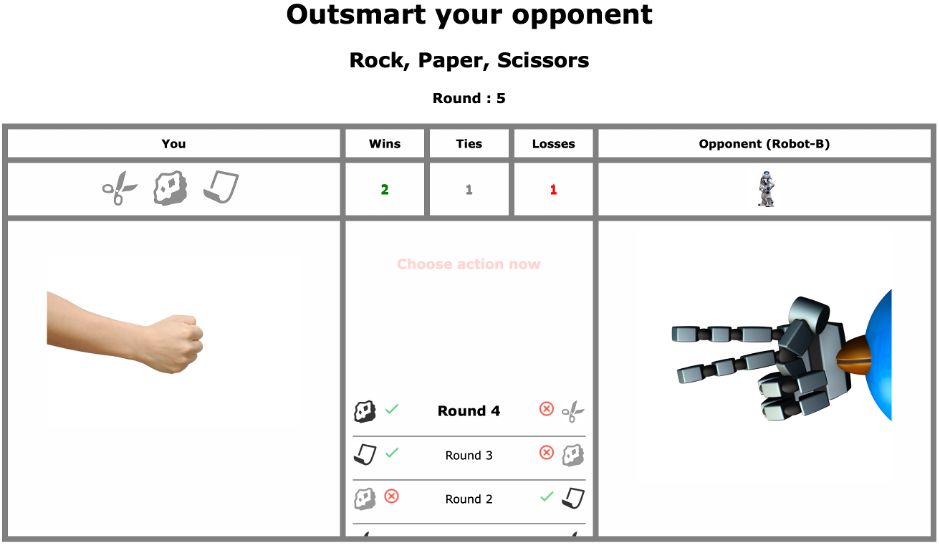
\includegraphics[width=\textwidth]{../images/feedback_rps} 

}

\caption{Screenshot of the Rock-Paper-Scissors game in Experiment 2. Shown here is the feedback stage, after both the human (left) and computer (right) players have chosen their action. The interface was similar in Experiment 1, but excluded the history of game play in the center panel.}\label{fig:feedback-rps-exp2}
\end{figure}

\begin{figure}

{\centering 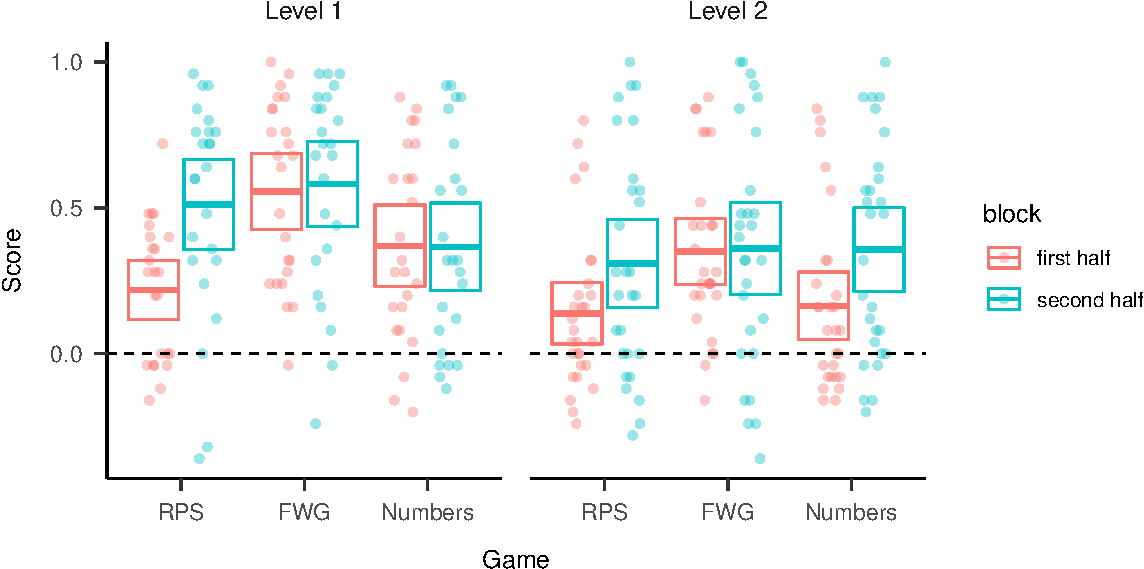
\includegraphics[width=\textwidth]{CBB_v2_files/figure-latex/exp1-avg-scores-game-1} 

}

\caption{Performance per game and block across conditions in Experiment 1. Points are scores of individual participants and boxes reflect the 95\% confidence intervals of the mean (center line equals the mean).}\label{fig:exp1-avg-scores-game}
\end{figure}

\hypertarget{behavioral-results}{%
\subsection{Behavioral results}\label{behavioral-results}}

Participants' scores in each half of each game are depicted in Figure
\ref{fig:exp1-avg-scores-game}. Overall, scores in each game were
significantly higher than 0, the expected score of uniformly random play
(RPS: \(M = 0.29\), 95\% CI \([0.21\), \(0.37]\), \(t(51) = 7.26\),
\(p < .001\); FWG: \(M = 0.45\), 95\% CI \([0.36\), \(0.54]\),
\(t(51) = 10.05\), \(p < .001\); Numbers: \(M = 0.31\), 95\% CI
\([0.22\), \(0.40]\), \(t(51) = 7.18\), \(p < .001\)). As uniformly
random play is the Nash equilibrium, this indicates successful deviation
from a Nash-optimal strategy. Additional analysis (see Supplementary
Information) indicates better performance against the level-1 compared
to level-2 opponent. This indicates that participants may have found it
more difficult to predict the actions of the more sophisticated level-2
opponent, even though both types of opponent are equally consistent and
hence equally exploitable in principle.

For an initial assessment of learning transfer, we focus on
participants' scores in the initial 5 rounds after the first round
(rounds 2-6) of each game (see Figure
\ref{fig:exp1-early-score-by-opp}). We exclude the first round as the
computer opponent played randomly here and there is no opportunity yet
for the human player to exploit their opponent's strategy. Players with
no knowledge of their opponent's strategy would be expected to perform
at chance level in these early rounds, whilst positive scores in rounds
2-6 are consistent with generalization of prior experience. The early
round score in both FWG and Numbers is significantly higher than 0 (FWG:
\(M = 0.24\), 95\% CI \([0.12\), \(0.36]\), \(t(51) = 4.13\),
\(p < .001\); Numbers: \(M = 0.15\), 95\% CI \([0.07\), \(0.24]\),
\(t(51) = 3.48\), \(p = .001\)). We did not expect positive early scores
for the RPS game, as it was the first game played and there was no
opportunity for learning about the opponent's strategy. Scores in this
game were indeed not significantly different from 0 (\(M = 0.06\), 95\%
CI \([-0.05\), \(0.18]\), \(t(51) = 1.08\), \(p = .285\)). Additional
analysis (see Supplementary Information) provided no evidence that
learning transfer differed between the two types of opponent.

\begin{figure}

{\centering 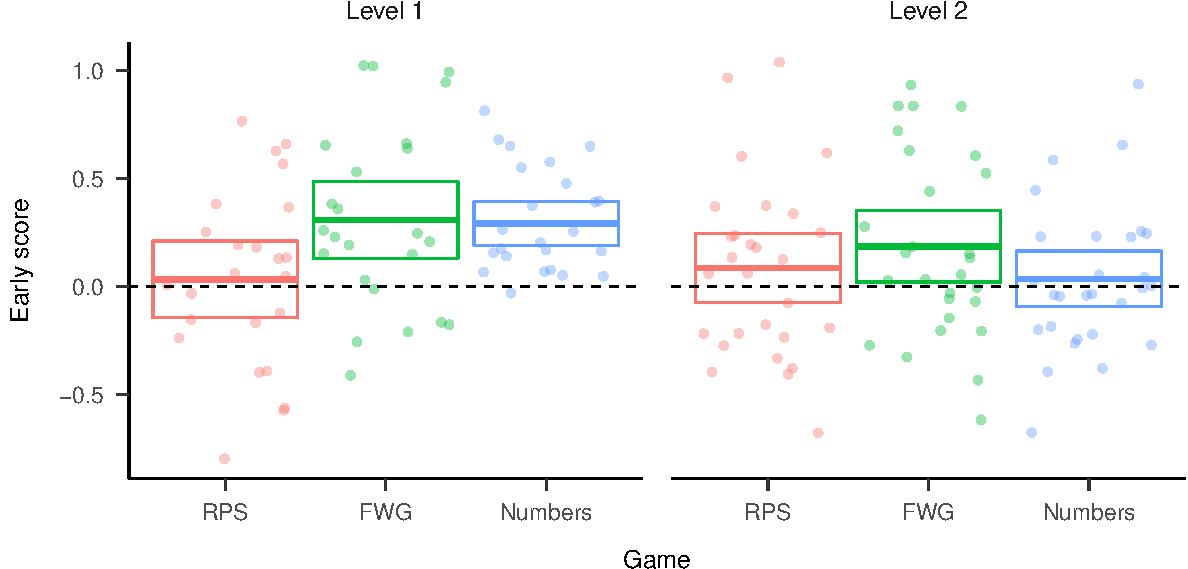
\includegraphics[width=\textwidth]{CBB_v2_files/figure-latex/exp1-early-score-by-opp-1} 

}

\caption{\label{ref:figure4-caption}Performance in early rounds (2-6) per game and block across conditions in Experiment 1. Points are scores of individual participants and boxes reflect the 95\% confidence intervals of the mean (center line equals the mean).}\label{fig:exp1-early-score-by-opp}
\end{figure}

\hypertarget{experiment-2}{%
\section{Experiment 2}\label{experiment-2}}

The results of Experiment 1 indicate that participants were able to
learn successful strategies which exploited the deviation from
Nash-optimal play of their opponents. Moreover, they were able to
transfer knowledge about their opponent to later games. In Experiment 2,
we aimed to obtain a stronger test of learning transfer. Instead of
facing a single level-1 or level-2 opponent throughout all games,
participants now faced both types of opponent. To perform well against
both opponents, participants would need to learn distinct strategies
against these opponents. To reduce effects of increased memory load due
to facing distinct opponents, we provided participants access to the
history of play against an opponent within each game (see Figure
\ref{fig:feedback-rps-exp2}). Finally, we changed the third game to a
penalty Shootout game, with participants aiming to score a goal and
opponents playing the role of goal keepers. Whilst this game has the
same number of actions as the first two (aim left, center, or right), it
is strategically dissimilar. Unlike the Numbers game in Experiment 1,
the Shootout game does not have a cyclical hierarchy between actions,
making it harder to win through a heuristic based on this cyclicity.

\hypertarget{methods-1}{%
\subsection{Methods}\label{methods-1}}

\hypertarget{participants-design}{%
\subsubsection{Participants \& Design}\label{participants-design}}

A total of 50 participants (21 females, 28 males, 1 unknown) were
recruited via the Prolific platform, none of which took part in
Experiment 1. The average age was 30.2 years, and the mean duration to
complete the task was 39 minutes. Participants received a fixed fee of
£2.5 for completing the experiment and a performance dependent bonus
(£1.32 on average).

\hypertarget{tasks-1}{%
\subsubsection{Tasks}\label{tasks-1}}

Participants played three games: Rock-Paper-Scissors (RPS),
Fire-Water-Grass (FWG), and the penalty Shootout game. The first two
games were identical to the ones used in Experiment 1. In the Shootout
game, participants took the role of the a football (soccer) player in a
penalty situation, with the computer opponent taking the role of the
goalkeeper. Players had the choice between three actions: shooting the
football to the left, right, or centre of the goal. Similarly, the
goalkeeper chooses between defending the left, right, or centre of the
goal. If participants shoot in a different direction than where the
goalkeeper defends, they win the round and the goalkeeper loses.
Otherwise, the goalkeeper catches the ball and the player loses the
round. There is no possibility of ties in this game. Figure
\ref{fig:screenshot-shootout} shows a snapshot of play in the Shootout
game. What makes this game different to the other games is that there
are now two ways to beat the opponent: if the shooter thinks their
opponent is going to choose to defend ``right'' in the next round, they
can win by either choosing to shoot ``left'' or ``center''. A level-1
shooter who thinks that their goalkeeper opponent will repeat their last
action has thus two possible best responses. A level-1 goalkeeper,
however, has only a single best response (defending where their opponent
aimed in the last round). A level-2 goalkeeper, who believes their
opponent is a level-1 shooter, will have two best responses however. We
programmed the level-2 computer player to choose randomly between these
two best responses.

As in Experiment 1, all the games have a unique mixed-strategy Nash
equilibrium consisting of uniformly random actions. If participants
follow this strategy, or simply don't engage in learning how the
opponent plays, they would score 0 on average against both level-1 and
level-2 players. Evidence of sustained wins would indicate that
participants have learned to exploit patterns in their opponents' play.

\begin{figure}

{\centering 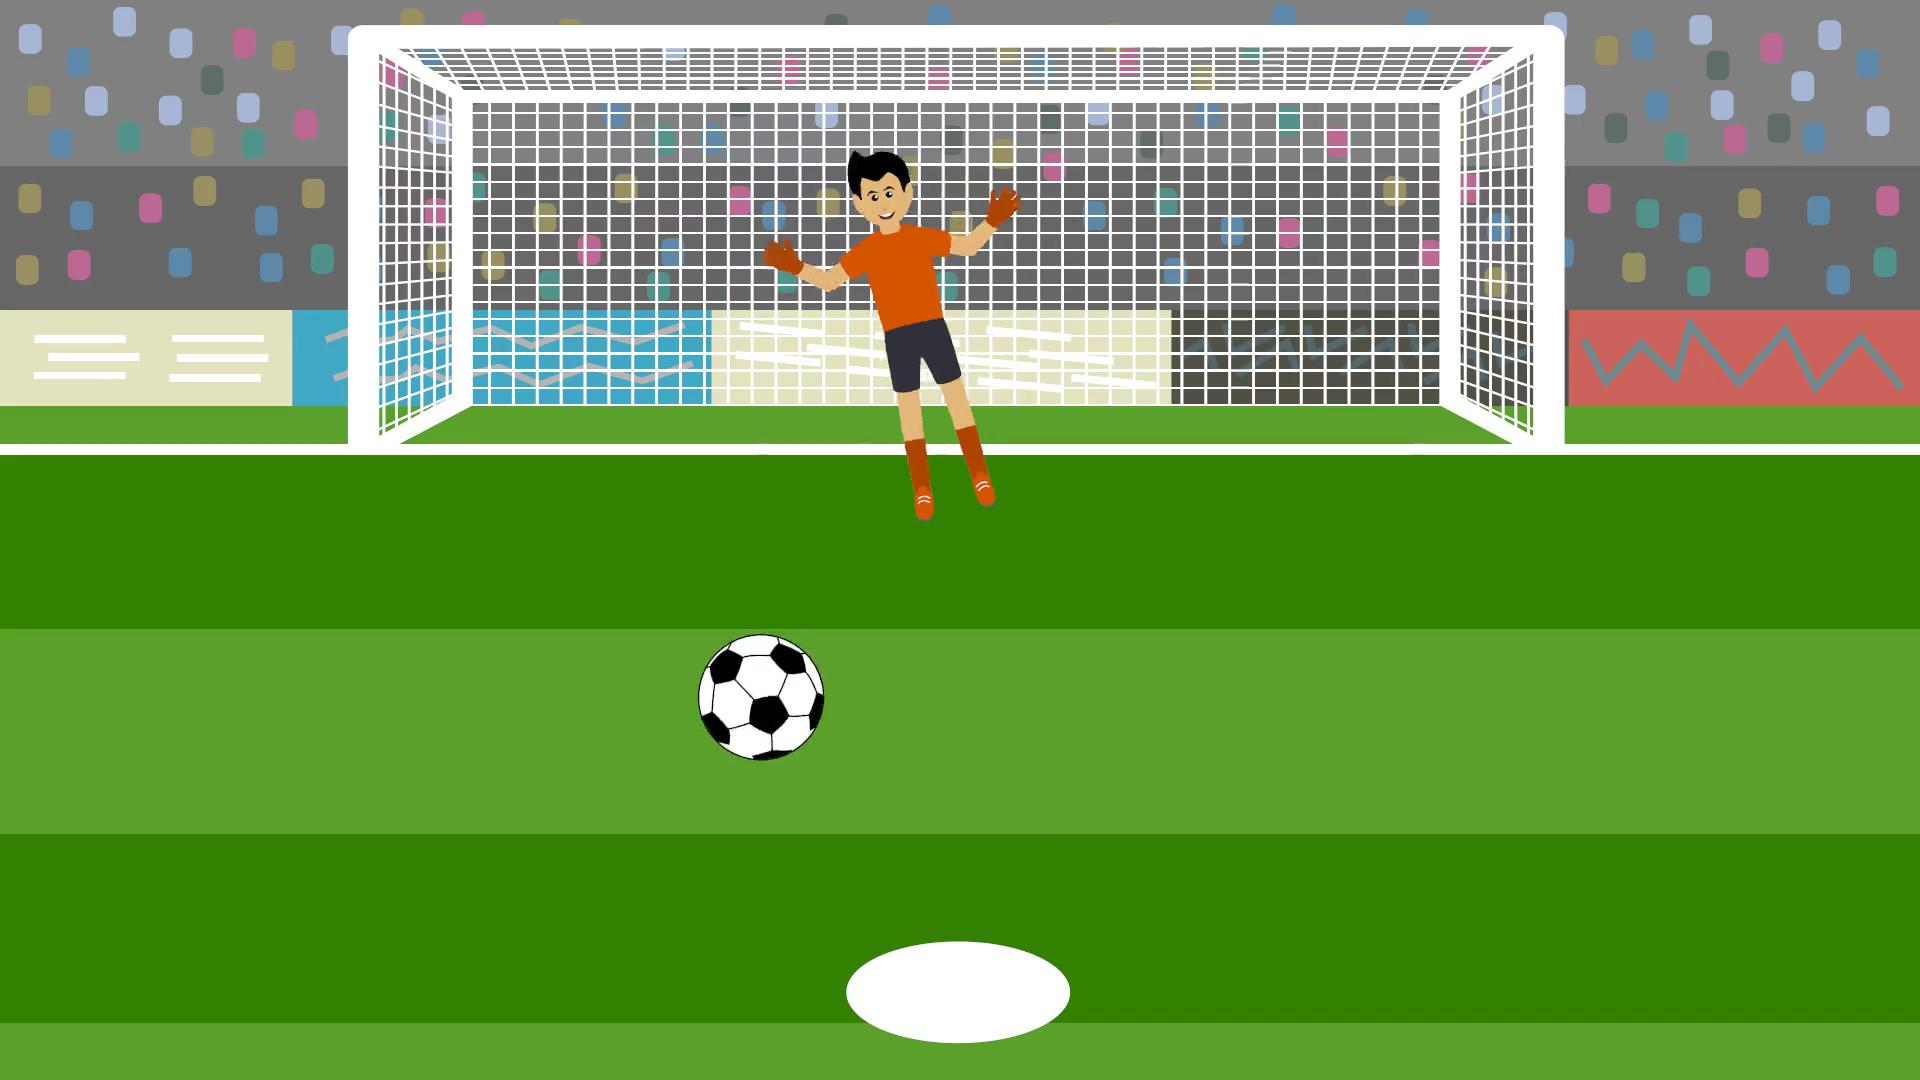
\includegraphics[width=\textwidth]{../images/shootout} 

}

\caption{Screenshot of the shootout game}\label{fig:screenshot-shootout}
\end{figure}

\hypertarget{procedure-1}{%
\subsubsection{Procedure}\label{procedure-1}}

Participants played 3 games sequentially against both level-1 and
level-2 computer opponents. As in Experiment 1, the computer opponents
retained the same strategy throughout the 3 games. Participants faced
each opponent twice in each game. Each game was divided into 4 stages,
numbered 1 to 4, consisting of 20, 20, 10, and 10 rounds respectively
for a total of 60 rounds per game. Participants started by facing one of
the opponents in stage one, then the other in stage two. This was
repeated in the same order in stages 3 and 4. Which opponent they faced
first was counterbalanced. All participants engaged in the three games
(RPS, FWG and Shootout) in this exact order, and were aware that their
opponent could not cheat and chose their action simultaneously with the
player, without knowing their choices beforehand. In order to encourage
participants to think about their next choice, a countdown timer of 3
seconds was introduced at the beginning of each round. During those 3
seconds, participants could not choose an action and had to wait for the
timer to run out. A random delay between 0.5 and 3 seconds was again
introduced before the choice of the computer agent was revealed, as a
way of simulating a real human opponent's decision time. After each
round, participants were given detailed feedback about their opponent's
action and whether they won or lost the round. Further information about
the history of play in previous rounds was also provided and
participants could scroll down to recall the full history of each
interaction against an opponent in a particular stage of a game. The
number of wins, losses and ties in each game were displayed at the top
of the screen, and this scoreboard was reinitialised to zero at the
onset of a new stage game.

\hypertarget{behavioral-results-1}{%
\subsection{Behavioral results}\label{behavioral-results-1}}

Participants' scores are depicted in Figure
\ref{fig:exp2-score-by-opp}.\footnote{Scores in the Shootout game were
  adjusted because there were 2 out of three possible winning actions in
  that game, compared to one out of three in RPS and FWG. As such, the
  expected score of random play in the Shootout game is 1/3, whilst it
  is 0 in the RPS and FWG game. To make the scores comparable, we
  therefore subtracted 1/3 from the Shootout scores.} Average (adjusted)
scores differed from 0 in all three games (RPS: \(M = 0.20\), 95\% CI
\([0.14\), \(0.27]\), \(t(49) = 6.26\), \(p < .001\); FWG: \(M = 0.28\),
95\% CI \([0.20\), \(0.36]\), \(t(49) = 7.25\), \(p < .001\); Shootout:
\(M = 0.35\), 95\% CI \([0.30\), \(0.41]\), \(t(49) = 13.62\),
\(p < .001\)). As in Experiment 1, this indicates that participants
successfully deviated from Nash-optimal (random) strategies. In contrast
to Experiment 1, additional analysis (see Supplementary Information)
showed no overall difference in performance between the two types of
opponent. However, participants performed better against the level-2
than level-1 opponent in RPG, but better against the level-1 opponent in
Shootout.

\begin{figure}

{\centering 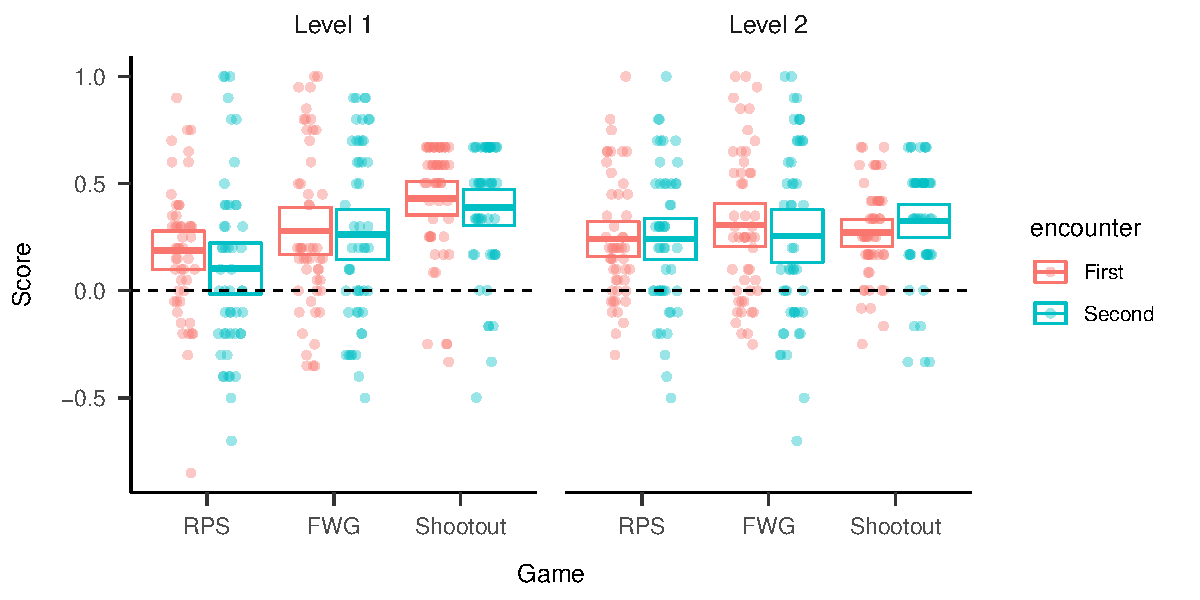
\includegraphics[width=\textwidth]{CBB_v2_files/figure-latex/exp2-score-by-opp-1} 

}

\caption{\label{fig:exp2-score-by-opp}Performance per game and interaction across opponents in Experiment 2. Points are scores of individual participants and boxes reflect the 95\% confidence intervals of the mean (center line equals the mean).}\label{fig:exp2-score-by-opp}
\end{figure}

As an initial assessment of transfer between games, we again focus on
participants' scores in rounds 2-6 of each game, both for stage 1 and 2
when participants first interact with an opponent in a game (see Figure
\ref{fig:exp2-early-score-by-opp}). We analyse these early-round scores
separately for each stage, as early-round scores in the second stage
could have benefited from experience in stage 1. Early-round scores
differed significantly from 0 for the both the FWG (stage 1:
\(M = 0.36\), 95\% CI \([0.24\), \(0.49]\), \(t(49) = 5.77\),
\(p < .001\); stage 2: \(M = 0.19\), 95\% CI \([0.07\), \(0.31]\),
\(t(49) = 3.15\), \(p = .003\)) and Shootout (stage 1: \(M = 0.30\),
95\% CI \([0.20\), \(0.40]\), \(t(49) = 5.90\), \(p < .001\); stage 2:
\(M = 0.28\), 95\% CI \([0.17\), \(0.40]\), \(t(49) = 4.98\),
\(p < .001\)). As expected, early scores in stage 1 of RPS did not
differ significantly from 0, \(M = 0.07\), 95\% CI \([-0.05\),
\(0.19]\), \(t(49) = 1.16\), \(p = .252\). In stage 2, however, they
did, \(M = 0.14\), 95\% CI \([0.02\), \(0.26]\), \(t(49) = 2.28\),
\(p = .027\). This indicates that the experience with the other opponent
in stage 1 may have provided an advantage to playing against a different
opponent in stage 2. Additional analysis (see Supplementary Information)
indicates transfer to the Shootout game may have been easier for the
level-1 than level-2 opponent. No reliable effect of stage was found.
The latter is important, because if early-round scores are due to
general practice effects rather then transfer of an opponent model, we
would expect early-round scores to increase between stage 1 and 2 in a
game.

\begin{figure}

{\centering 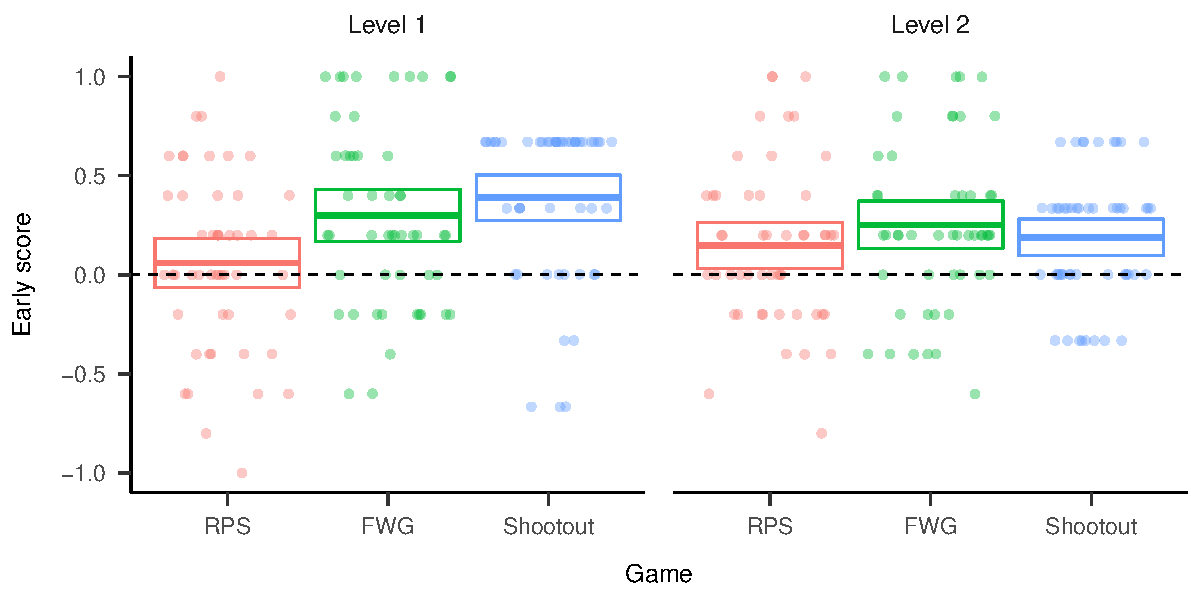
\includegraphics[width=\textwidth]{CBB_v2_files/figure-latex/exp2-early-score-by-opp-1} 

}

\caption{\label{ref:figure4-caption}Performance in early rounds (2-6) per game and opponent in Experiment 2. Points are scores of individual participants and boxes reflect the 95\% confidence intervals of the mean (center line equals the mean).}\label{fig:exp2-early-score-by-opp}
\end{figure}

\hypertarget{computational-modelling}{%
\section{Computational modelling}\label{computational-modelling}}

The results of Experiment 2 confirm findings from Experiment 1 on
learning transfer in a situation where participants need to learn about
two distinct opponents. In both Experiment 1 and 2, participants adapted
their strategies to level-1 and level-2 opponents to exploit deviations
from Nash-optimal play. Moreover, from early-round performance, we found
initial evidence that knowledge about both types of opponents was
transferred to similar (FWG) and dissimilar (Numbers or Shootout) games.

To gain more insight into how participants adapted their strategies to
their computer opponents, we constructed and tested several
computational models of strategy learning. The baseline model assumes
play is random, and each potential action is chosen with equal
probability. Note that this corresponds to the Nash equilibrium
strategy. The other models adapted their play to the opponent, either by
reinforcing successful actions in each game (reinforcement learning), or
by determining the type of opponent through Bayesian learning (Bayesian
Cognitive Hierarchy models). We also include the (self-tuning) Expected
Weighted Attraction (EWA) model, which is a popular model in behavioural
economics.

In the following, we will describe the models in more detail, and
provide some intuition into how they implement learning about the game
and/or the opponent. Throughout, we use the following notation: In each
game
\(g \in \{\text{RPS},\text{FWG}, \text{Numbers}, \text{Shootout} \}\),
on each trial \(t\), the participant chooses an action
\(a_t \in \mathcal{A}_g\), and the opponent chooses action
\(o_t \in \mathcal{A}_g\), where \(\mathcal{A}_g\) is the set of allowed
actions in game \(g\), e.g. \(\mathcal{A}_\text{RPS} = \{R,P,S\}\). The
participant then receives reward \(r_t \in \{1,0,-1\}\), and the
opponent receives \(-r_t\). We use the state variable
\(s_t = \{a_{t-1},o_{t-1}\}\) to denote the actions taken in the
previous round \(t-1\) by the participant and opponent. The initial
state is empty, and we assume that the action at a first encounter of an
opponent in a game is chosen at random.

\hypertarget{reinforcement-learning-rl-model}{%
\subsection{Reinforcement learning (RL)
model}\label{reinforcement-learning-rl-model}}

We first consider a model-free reinforcement learning algorithm, where
actions that have led to positive rewards are reinforced, and the
likelihood of actions that led to a negative reward is lowered. Since
the computer players in this experiment based their play on the actions
in the previous round, a suitable RL model for this situation is one
which learns the value of actions contingent on plays in the previous
round, i.e.~by defining the state \(s_{t}\) as above. The resulting RL
model learns a \(Q\)-value (Watkins and Dayan 1992) for each
state-action pair:
\[Q_{t+1}(s_{t},a_{t}) = Q_{t}(s_{t},a_{t}) + \alpha \left( r_{t}  - Q(s_{t},a_{t}) \right) ,\]
where \(Q(s_{t},a_{t})\) is the value of taking action \(a\) when in
state \(s\) at time \(t\), and \(\alpha \in [0,1]\) the learning rate.
For instance, \(Q_t(\{R,S\},P)\) denotes the value of taking action
``Paper'' this round if the player's last action was ``Rock'' and the
opponent played ``Scissors''. Actions are taken according to a softmax
rule: \begin{equation}
\label{eq:softmax}
P_{t}(a|s_t) = \frac{\exp \{ \lambda Q_{t}(a,s_t) \}}{\sum_{a' \in \mathcal{A}_g} \exp \{\lambda  Q_{t}(a',s_t) \}}, 
\end{equation} where the inverse temperature parameter \(\lambda\)
determines the consistency of the strategy (the higher \(\lambda\), the
more often the action with the highest \(Q\)-value is chosen). While
this RL model allows the players to compute the values of actions
conditional on past play, crucially, it will not be able to transfer
learning between games, as each game has a different state space
\(\mathcal{S}_g\) and action space \(\mathcal{A}_g\), and there is no
simple way to map states and actions across games. The RL model has two
free parameters: the learning rate (\(\alpha\)) and the inverse
temperature (\(\lambda\)).

\hypertarget{experience-weighted-attraction-ewa-model}{%
\subsection{Experience-weighted attraction (EWA)
model}\label{experience-weighted-attraction-ewa-model}}

As discussed in the introductory section on computational models, the
self-tuning Experience Weighted Attraction (EWA) model combines two
seemingly different approaches, namely reinforcement learning and belief
learning. The EWA model is based on updating ``Attractions'' for each
action over time given a particular state. The attraction of action
\(a\) at time \(t\) given state \(s\) is denoted as \(Q_{t}(a, s)\) and
updated as
\[ Q_{t+1}(a,s) =  \frac{\phi(t) \ N(t) \ Q_{t}(a,s) + [ \delta_{a}(t) + (1-\delta_{a}(t)) \ I(a_t = a )] \ R(a,o_t) } {\phi(t)N(t) + 1} ,\]
where \(I(x)\) is an indicator function which takes the value 1 if its
argument is true and 0 otherwise, and \(R(a,o_t)\) is the reward that
would be obtained from playing action \(a\) against opponent action
\(o_t\). \(R(a,o_t)\) equals the actual obtained reward when
\(a = a_t\), and otherwise is a counterfactual reward that would have
been obtained if a different action were taken. Unlike reinforcement
learning, this uses knowledge of the rules of the game to allow
reinforcing actions that were not actually taken by the rewards they
would have provided. The parameter \(\delta\) reflects the weight given
to such counterfactual rewards. Setting \(\delta = 0\) leads to
reinforcement only of actions taken, while positive values of \(\delta\)
makes the update rule take into account foregone payoffs, which is
similar to weighted fictitious play (Cheung and Friedman 1994). \(N(t)\)
represents an experience weight and can be interpreted as the number of
``observation-equivalents'' of past experience. We initialise it to 1 so
initial attractions and reinforcement from payoffs are weighted equally.

In the earlier version of the EWA model (Camerer and Hua Ho 1999),
\(\phi\) and \(\delta\) were time-invariant free parameters. In the
self-tuning EWA model (Ho, Camerer, and Chong 2007), the values of
\(\delta\) and \(\phi\) are learnt from experience. Over time,
\(\delta\) is updated as
\[\delta_{a}(t) = \begin{cases} 1 & \text{if }  R(a,o_{t}) \geq r_{t}  \\
0 & \text{otherwise} \end{cases}\] The \(\phi_{t}\) parameter can be
interpreted as a discount of prior experience, modelling either limited
agent memory or changes in the game conditions. At the core, \(\phi(t)\)
depends on a surprise index \(S_{p}(t)\):
\[\phi(t) = 1 - \frac{1}{2}S_{p}(t) ,\] where \(S_{p}(t)\) quantifies
how the opponent deviates from past play. It is calculated in turn
through the cumulative history of play, across opponent possible actions
k, as \(h^{k}(t)\):
\[h^{k}(t)= \frac{ \sum_{\tau = 1}^t  I( o_{\tau} = o^k )} {t}, \] as
well as an indicator vector of the most recent opponent play:
\[r^k(t) = I(o^k=o_{t}), \] Where \(I\) is the indicator function as
defined above. To get the surprise index, we simply sum all the squared
deviations between the cumulative history vector \(h^{k}(t)\) and the
immediate history \(r^k(t)\):
\[S_{p}(t) = \sum_{k=1}^{|\mathcal{A}_g|} (h^{k}(t) - r^k(t))^2 \] For
more details on the self-tuning EWA model, we refer the reader to (Ho,
Camerer, and Chong 2007). As in the RL model above, actions are chosen
based on a softmax decision rule (Equation \ref{eq:softmax}). The
self-tuning EWA has one free parameter: the inverse temperature of the
softmax decision rule (\(\lambda\)).

\hypertarget{bayesian-cognitive-hierarchy-bch-model}{%
\subsection{Bayesian Cognitive Hierarchy (BCH)
model}\label{bayesian-cognitive-hierarchy-bch-model}}

In what we call the Bayesian Cognitive Hierarchy (BCH) model, the
participant attempts to learn the type of opponent they are facing
through Bayesian learning. For present purposes, we assume participants
consider the opponent could be either a level 0, level 1, or level 2
player, and start with a prior belief that each of these types is
equally likely. They then use observations of the opponent's actions to
infer a posterior probability of each type:
\[P(\text{level}=k | \mathcal{D}_{t})  \propto  P(\mathcal{D}_{t}|\text{level}=k ) \times P(\text{level}=k) ,\]
where \(\mathcal{D}_{t} = \{s_1,\ldots,s_t\}\) is the data available at
time \(t\). The likelihood is defined as
\[P(\mathcal{D}_{t}|\text{level}=k) = \prod_{j=1}^t \left( \theta \frac{1}{|\mathcal{A}_g|} + (1-\theta) f_k(o_j|s_{j})\right) ,\]
where \(f_k(o_t|s_{t}) = 1\) if \(o_t\) is the action taken by a level
\(k\) player when the previous round play was
\(s_t = (a_{t-1}, o_{t-1})\), and 0 otherwise. Note that the likelihood
assumes (correctly) that there is a probability \(\theta \in [0,1]\)
that the opponent takes a random action. The posterior at time \(t-1\)
forms the prior at time \(t\). The probability that an action \(a\) is
the best response on trial \(t\) is defined as:
\[B_t(a) = \sum_{k = 0}^2 \sum_{o \in \mathcal{A}_g} b(a,o) f_k(o|s_{t})  P(\text{level}=k|\mathcal{D}_{t-1}), \]
where \(b(a,o) = 1\) if action \(a\) is a best response to opponent's
action \(o\) (i.e.~it leads to a win).

We assume participants choose actions through a softmax over these
probabilities of best responses:
\[P_t(a|s_t) = \frac{\exp\{\lambda B_t(a) \}}{\sum_{a' \in \mathcal{A}_g} \exp \{ \lambda B_t(a')\}}.\]

Unlike the models above, the BCH model allows for between-game transfer,
as knowledge of the level of the opponent can be used to generate
predictions in games that have not been played before. This
generalization is done simply by using the posterior
\(P(\text{level} = k|\mathcal{D}_T)\) from the previous game as the
prior distribution in the next game. However, the participant might also
assume that the level of reasoning of their opponent does not generalize
over games. This would mean starting with a ``fresh'' prior
\(P(\text{level} = k)\) at the start of each game. We hence distinguish
between two versions of the BCH model. In the No-Between-Transfer
(BCH\_NBT) variant, participants assume a uniform probability of the
different levels at the start of each game (and hence do not transfer
knowledge of their opponent between games). In the Between-Transfer
model (BCH\_BT), participants use the posterior probability over the
levels of their opponent as the prior at the start of a new game
(i.e.~complete transfer of the knowledge of their opponent). Both
versions of the BCH model have two free parameters: the assumed
probability that the opponent chooses a random action (\(\theta\)), and
the temperature parameter of the softmax function (\(\lambda\)).

\hypertarget{estimation}{%
\subsection{Estimation}\label{estimation}}

For both experiments, we fitted all models to individual participant
data by maximum likelihood estimation using the DEoptim R package
(Mullen et al. 2011). We use the Bayesian Information Criterion (BIC) to
determine the best fitting model for each participant. For Experiment 1,
we fitted a total of 5 models: a baseline model assuming random play
(Nash), the Bayesian Cognitive Hierarchy model allowing transfer between
games (BCH\_BT) and without transfer between games (BCH\_NT), as well as
a reinforcement learning (RL), and finally a self-tuning EWA model with
the same state space (EWA). In Experiment 2, because participants were
interacting with each opponent twice within each game, we need to
distinguish between two types of opponent model transfer. We can have
transfer \emph{within} games between the first and second interaction
with the opponent. In addition, we can also have transfer \emph{between}
games, as in e.g.~transferring a learned opponent model from RPS to FWG.
Therefore, we fitted a total of three versions of the Bayesian Cognitive
Hierarchy model: BCH\_BT allows for both within and between game
transfer (between game transfer without within game transfer is
implausible); BCH\_WT allows only for within-game transfer, but not
between game transfer; BCH\_NT allows for no transfer within or between
games. As the RL model can't account for between game transfer due to a
change in state and action space, we can only have models that allowing
for within game transfer (RL\_WT) or with no transfer within games
(RL\_NT). Likewise, we fit both a self tuning EWA model with (EWA\_WT)
and without (EWA\_NT) within-game transfer. Including the baseline model
of random play (Nash), we therefore fitted a total of 8 models for
Experiment 2.

\hypertarget{model-comparison}{%
\subsection{Model comparison}\label{model-comparison}}

When considering which single model fits participants behaviour over the
whole experiment best, we find that in both experiments the RL model
outperforms the other models, followed by the random (Nash) model
(Figure \ref{fig:exp-comp-models}). Relatively few participants were
best described by one of the BCH models or the EWA model.

\begin{figure}

{\centering 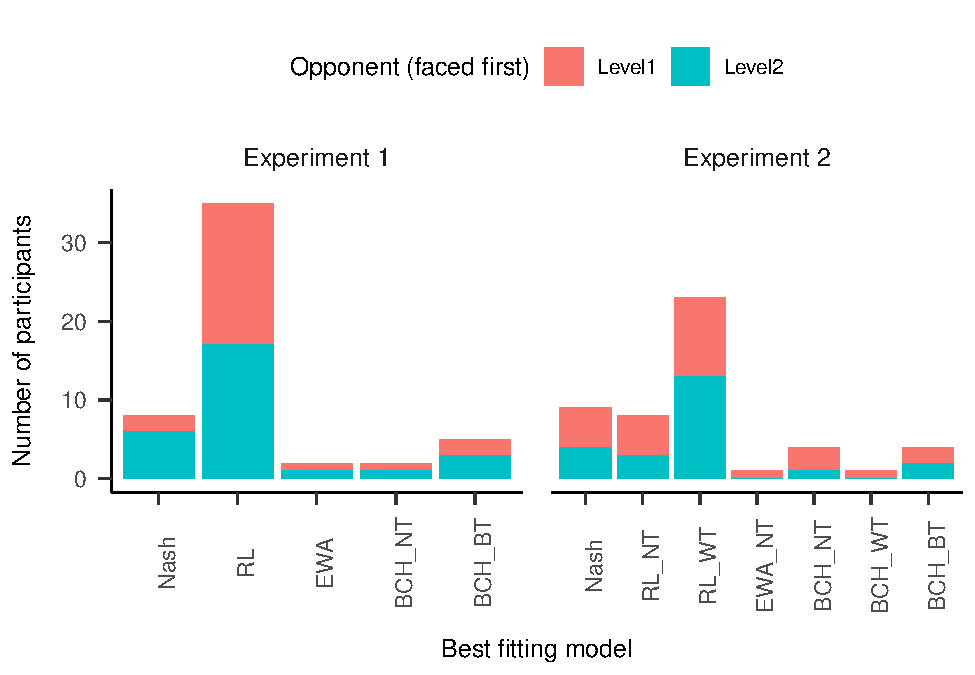
\includegraphics[width=\textwidth]{CBB_v2_files/figure-latex/exp-comp-models-1} 

}

\caption{Number of participants best fitted by each model  in Experiment 1 and 2 according to the BIC. Results are seperated by opponent (Experiment 1) and which opponent they faced first (Experiment 2).}\label{fig:exp-comp-models}
\end{figure}

As the RL models don't transfer learning between games, this is at odds
with the behavioural results, which showed evidence for such transfer.
In order to investigate this discrepancy further, we plot the likelihood
by trial for each game and three strategies: reinforcement learning
(RL), Bayesian Cognitive Hierarchy with between-game transfer (BCH\_BT),
and the random (Nash) strategy. Figure \ref{fig:exp1-lik-by-tr} shows
that in the initial rounds of the the later games in Experiment 1, the
likelihood for the BCH model is higher than that of the other two
models. However, over time, the likelihood of the RL model increases and
exceeds that of the BCH model. The same pattern holds for Experiment 2
(Figure \ref{fig:exp2-lik-by-tr}). Again, the BCH\_BT model with
between-game transfer has the highest likelihood in the early stages of
the later games (apart from stage 1 of the Shootout game, where the RL
model is better). In later rounds, the likelihood of the RL model
exceeds that of the BCH model.

The fact that the likelihoods of the main strategies considered cross
over in both experiments is consistent with participants switching
between strategies as the games progress. According to this
interpretation, participants base their responses in early rounds on the
learned level of their opponents iterative reasoning, switching later to
learning good actions through reinforcement. We initially did not
predict this strategy switching. Whilst the likelihoods are suggestive,
we sought an approach to formally test for strategy switching.

\hypertarget{hidden-markov-model-analysis-of-strategy-switching}{%
\subsection{Hidden Markov model analysis of strategy
switching}\label{hidden-markov-model-analysis-of-strategy-switching}}

\begin{figure}

{\centering 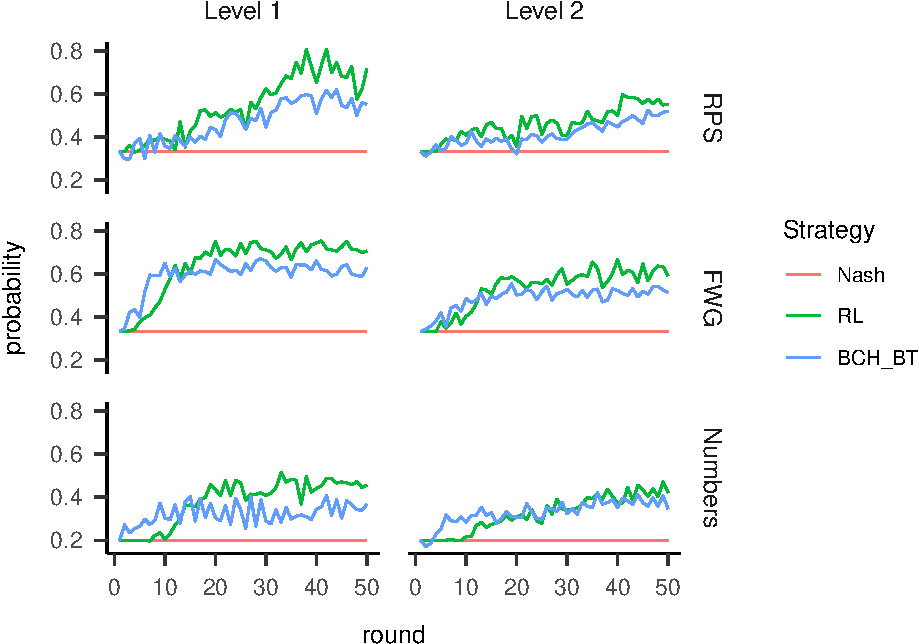
\includegraphics[width=\textwidth]{CBB_v2_files/figure-latex/exp1-lik-by-tr-1} 

}

\caption{Average likelihood of the random (Nash), reinforcement learning (RL) and Bayesian Cognitive Hierarchy model by trial, game, and opponent faced in Experiment 1.}\label{fig:exp1-lik-by-tr}
\end{figure}

\begin{figure}

{\centering 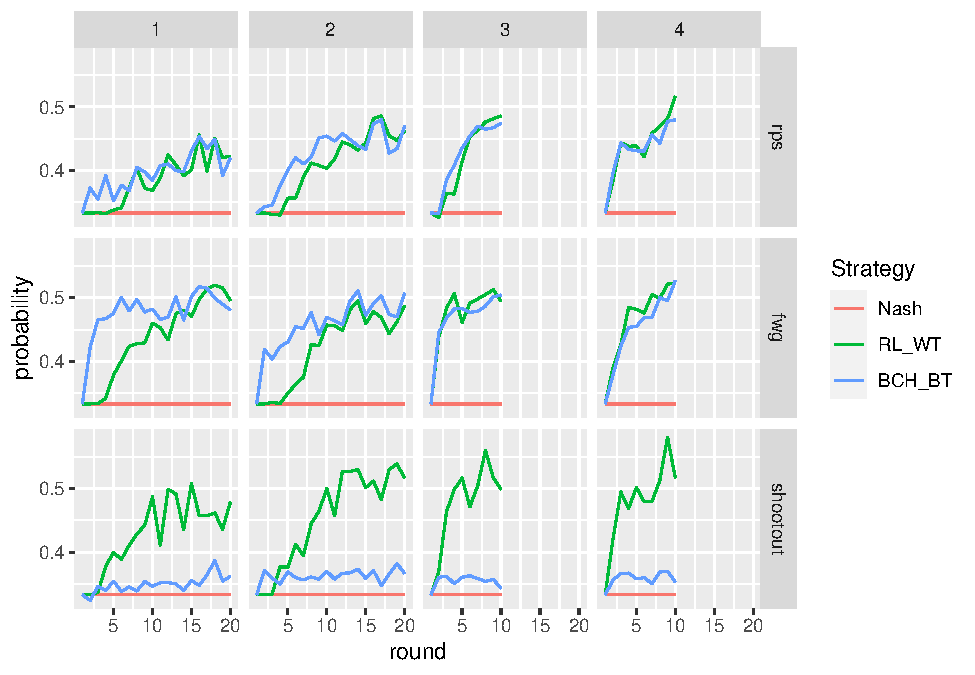
\includegraphics[width=\textwidth]{CBB_v2_files/figure-latex/exp2-lik-by-tr-1} 

}

\caption{Average likelihood of the random (Nash), reinforcement learning (RL) and Bayesian Cognitive Hierarchy model by trial, stage, and game in Experiment 2.}\label{fig:exp2-lik-by-tr}
\end{figure}

We use hidden Markov models to test for strategy switching in
participants' play. In these models, the three strategies (RL, BCH with
between-game transfer, and Nash) correspond to latent states which
determine the overt responses (actions chosen). The models allow for
switching between the states (i.e.~strategies) over time. Hidden Markov
models assume that an observable action at time \(t\) depends on a
latent state at time \(t\). It is assumed that the latent state at time
\(t\) depends on the latent state at the previous time \(t-1\). The
model is specified by the state-conditional action distributions (these
are provided by the likelihood of the fitted models), an initial state
distribution (the distribution over the strategies at the initial
round), and the state-transition probabilities (probability of switching
from one state/strategy to another). Initial state probabilities and the
transition probabilities were estimated with the depmixS4 package
(Visser and Speekenbrink 2010). As a statistical test of strategy
switching, we compare the hidden Markov model to a constrained version
which assumes the probability of switching from one strategy to a
different one is 0. This model thus assumes that when players start with
a particular strategy, they continue using it throughout the experiment.

\begin{figure}

{\centering 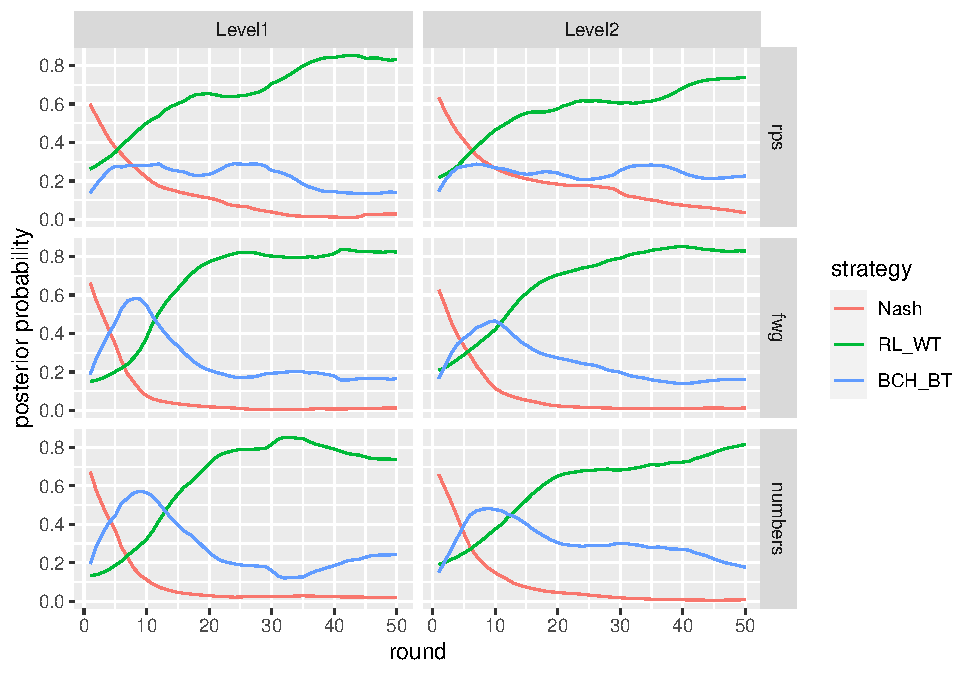
\includegraphics[width=\textwidth]{CBB_v2_files/figure-latex/exp1-posteriors-plot-1} 

}

\caption{Average posterior probability of each strategy by trial, game and opponent faced, in Experiment 1.}\label{fig:exp1-posteriors-plot}
\end{figure}

In Experiment 1, a likelihood-ratio test shows that the HMM model with
switching fits significantly better than the non-switching one,
\(\chi^2(6) = 211.09\), \(p < .001\). We should note that as the no
switch model involves restricting parameters of the switching model on
the bounds of the parameter space, the \(p\)-value of this test may not
correspond to the true Type-1 error rate. We therefore also consider
model selection criteria. These also show that the switching model (AIC
= 14636.87, BIC = 14692.56) fits better than the non-switching model
(AIC = 14835.96, BIC = 14849.88). This provides further statistical
evidence in favour of the hypothesis that participants switch between
strategies. Figure \ref{fig:exp1-posteriors-plot} depicts the average
posterior probability of each strategy, as a function of trial and
opponent faced. As can be seen, there is evidence of strategy switching
in the FWG and Numbers games: Initially, participants appear to use a
random strategy (in the first round of a game, there is no way to
predict the opponent's action), after which the BCH strategy becomes
dominant. In the later rounds of the games, the RL strategy becomes
dominant, however.

\begin{figure}

{\centering 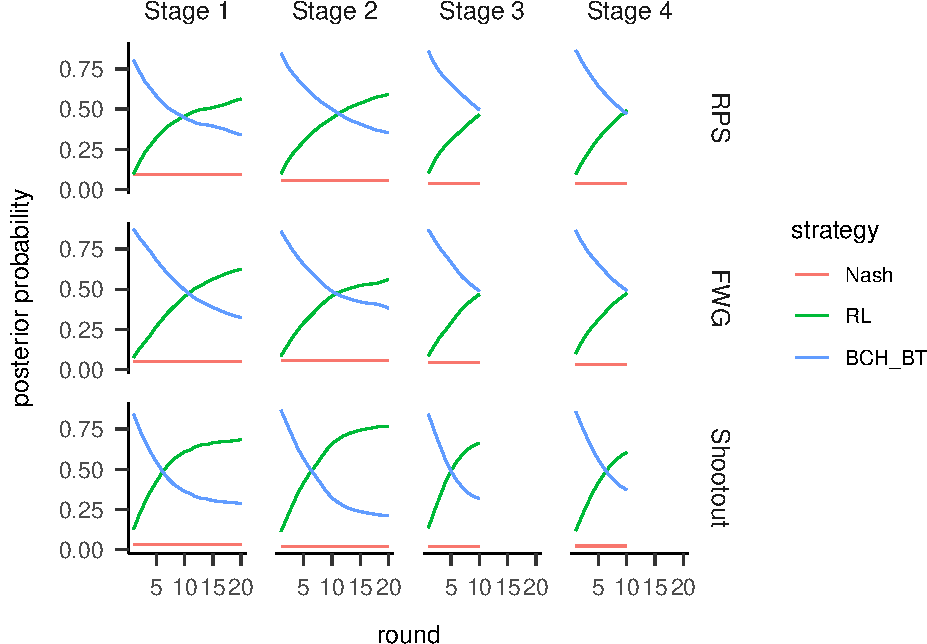
\includegraphics[width=\textwidth]{CBB_v2_files/figure-latex/exp2-posteriors-plot-1} 

}

\caption{Average posterior probability of each strategy by trial, stage, and game in Experiment 2.}\label{fig:exp2-posteriors-plot}
\end{figure}

In Experiment 2, the switching model (AIC = 16879.97, BIC = 16936.81)
again fits better than the restricted non-switching model (AIC =
16938.41, BIC = 16952.62), \(\chi^2(6) = 70.44\), \(p < .001\). The
posterior probabilities of the strategies (Figure
\ref{fig:exp2-posteriors-plot}) show very clear evidence of strategy
switching across games and stages, from using a BCH model in the initial
rounds to an RL strategy later on.

\hypertarget{discussion}{%
\section{Discussion}\label{discussion}}

In this study, we investigated human learning transfer across games by
making human participants play against computer agents with limited
levels of iterated reasoning. We were interested in whether participants
learn about the strategy of their opponent and transfer such knowledge
between games.

The results of our first experiment show that the majority of
participants learnt to adapt to their opponent's strategy over multiple
rounds of the Rock-Paper-Scissors (RPS) game, and generalised this
learning to a similar (Fire-Water-Grass) and less similar (Numbers)
game. In the second experiment, participants faced both types of
opponents, allowing for a stronger test of opponent modelling, as
participants would need to learn a different strategy for each opponent.
In Experiment 1, participants could learn a single strategy for each
game, making opponent modelling possibly less pertinent. In Experiment
2, we again found clear evidence of transfer in the early rounds of the
later games.

What exactly did the players learn in the first game (RPS) that allowed
them to beat their opponent in the later games (FWG, and Numbers or
Shootout)? What did the players learn specifically about their
opponent's strategy and what form did this learning take? One possible
answer is that participants learned simple rules based on last round
play. For instance, ``play Scissors whenever my opponent played Rock in
last round'', or ``play Paper whenever the last round play was either
Rock or Scissors''. These are the type of strategies that are learned by
the model-free reinforcement learning we used in our computational
modelling. While this strategy fitted participants' actions the best
overall, there are at least two reasons why this account is not
satisfactory as a complete description of participants' behaviour.
Firstly, the learned strategies are not transferable to new games. There
is no simple way to map ``play Scissors whenever my opponent played Rock
in last round'' in the RPS game to ``play Grass whenever my opponent
played Fire in last round''. Such a mapping may be possible by
translating the rules and structure from RPS to FWG, but model-free
reinforcement learning lacks the tools to do this: Model-free
reinforcement learning would need to start from scratch in each new
game, yet we found evidence that participants could successfully exploit
their opponent's strategy in early rounds of new games. Secondly, a
reinforcement learning strategy would fare equally well against the
level-1 and level-2 opponent. Whilst choosing different actions, the
contingency between the state (last round play) and actions is the same
for both opponents. Yet, in Experiment 1, we found that participants
performed better against the level-1 opponent compared to the level-2
opponent. The difference in performance between the two types of
opponent indicates that the actions of the more sophisticated level-2
opponent, or the best response to these, were somehow more difficult to
predict.

We are left with two possible explanations: First, it is possible that
participants discovered a heuristic that allowed them to beat their
opponent without explicitly modelling their strategy, and that this
heuristic is transferable to new games. Because of the cyclicity in
action choices (e.g., Rock beats Scissors, Scissors beats Paper, Paper
beats Rock), it is possible to beat a level-2 opponent most of the time
by following a simple rule: Play in the next round whatever the opponent
played in the last round. This is a rule that wins and is transferable
to other games, as it does not depend on action labels. In the same
vein, a heuristic that beats a level-1 player can be stated as ``Choose
the action that would have been beaten by my previous action''.
Intuitively, it seems that the heuristic for a level-2 player is simpler
than that for a level-1 player, which is at odds with the finding that
participants performed better against the level-1 opponent.

A second explanation is that participants engaged in iterative
reasoning, inferring their opponent's beliefs and countering the
resulting actions. For instance, this would be reasoning of the form
``My opponent expects me to repeat my last action, choosing an action
that would beat my last action. Hence, I will choose the action that
beats their best response'' or ``My opponent thinks I expect them to
repeat their action, hence expecting me to choose the action that beats
their last action. They will therefore choose the action that beats this
one, and hence I should choose the action that beats their best
response.'' Beating a level-1 player, in this account, requires being a
level-2 player, and beating a level-2 player requires being a level-3
player. Intuitively, the additional step of iterative reasoning involved
in beating a level-2 player makes the level-3 strategy more demanding
and difficult to implement, which is consistent with the lower
performance against the level-2 opponent. We did not find a clear
difference in performance against the two opponents in Experiment 2,
where participants faced both consecutively. Learning about the distinct
strategies of two different opponents is likely more difficult than
learning about a single opponent. And switching between opponents may
place additional demands on memory and impose task switching costs.
These factors may have masked the performance difference found in
Experiment 1. Nevertheless, we found that participants learned to
successfully exploit the strategies of both players in Experiment 2, as
well as transferring their learning to new games.

The difference in performance against the two opponents, coupled with
evidence for successful transfer, point to participants engaging in
iterative reasoning and learning something useful about their opponent's
limitations in this regard. This is the type of learning encapsulated by
our Bayesian Cognitive Hierarchy model. It involves the evaluation of
explicit hypotheses and results in better problem-solving skills
(Mandler 2004). Since it is less context dependent, this type of
learning is generalizable to new situations, akin to the more general
framework of rule-based learning explored by Stahl (Stahl 2000, 2003).
When asked to describe the strategy of their opponents at the end of the
study, many participants made reference to a form of recursive
reasoning, which provides additional support for this account.

We admit that our implementation in the BCH models does not predict a
performance difference between the types of opponents. Starting with an
equal prior belief over the different levels of sophistication, a BCH
player would perform equally well against the level-1 and level-2
opponent. There are two routes to explain the difference in performance.
Firstly, prior beliefs might be biased against higher-level opponents
(i.e., participants might have believed it is more likely that they
would face level-1 opponent than a level-2 opponent). Secondly, if the
actions of a level-2 opponent are more difficult to predict than those
of a level-1 opponent, this might introduce more noise in the likelihood
of the opponents actions given their level of sophistication. Either of
these mechanisms would explain why learning the strategy of the level-2
opponent is more difficult and slower than learning the strategy of the
level-1 opponent.

Using hidden Markov models, we found evidence of strategy switching
between the BCH and RL strategies, and such switching seems more
consistent with the latter idea. If predicting an opponent's actions
through iterative reasoning is cognitively demanding and error-prone, it
is resource-rational to switch to less costly yet equally successful
strategies when these are available (Lieder and Griffiths 2020).
Initially, a model-free reinforcement learning strategy will be less
successful than an iterative reasoning one. However, given enough
experience, it will be on par with an iterative reasoning strategy. As
it involves simple state-action contingencies, a model-free RL strategy
may also be computationally less costly, making it overall more
effective to rely on this than iterative reasoning. This is similar to
the arbitration between model-free and model-based RL (Daw, Niv, and
Dayan 2005; Simon and Daw 2011; Wouter Kool 2011). In repeated and
well-practised situations, relying on habits allows one to save
cognitive resources for other demands. However, when the environment --
or game -- changes, it is prudent to use all available resources to
reorient oneself.

A limitation of the design of both experiments is that the order of the
games was not counterbalanced. We chose the order used as we believed it
would be most conducive to learning the strategy of the opponent.
Starting with a familiar game (RPS) would allow participants to focus on
how their opponent plays, rather than also having to learn the rules of
the game. A new but isomorphic game (FWG) allows for the most
straightforward transfer. We reasoned that transfer to a less similar
game (Numbers of Shootout), a stronger test of generalization, would be
more likely given sufficient experience in two similar games.
Determining the level of iterative reasoning in these latter games is
more difficult (the Numbers game has many ties, whilst in Shootout
actions are often consistent with different level-\(k\) opponents).
Counterbalancing the order of the games would mean many participants
would start with these more difficult games. Whilst we believe these
games are good candidates for testing generalisation of previously
learned opponent models, they are poor environments to learn them in the
first place. Since participants can't transfer what they have not
learned, we expect that starting with these games might prohibit
learning opponent models and thus their transfer. However, we can't rule
out that part of the transfer effects found for early round scores is
due to general practice effects, or differences in the difficulty of the
games. We find it unlikely that the transfer effects we found are
entirely due to such confounded practice or difficulty effects. Firstly,
general practice or difficulty effects should not depend on the level of
the opponent. However, we found evidence that overall scores (Experiment
1) and early round scores (Experiment 2) differed between the two types
of opponents. Secondly, practice effects would be evident within a game,
but we found no main effect of stage on early-round scores in Experiment
2.

\hypertarget{conclusion}{%
\section{Conclusion}\label{conclusion}}

In two experiments we found that people successfully deviate from Nash
equilibrium play to exploit deviations from such play by their
opponents. Moreover, people can transfer knowledge about the underlying
limitations of their opponents' degree of iterative reasoning to new
situations. Within games, we found evidence that people start new games
with a reasoning-based strategy that allows them to transfer knowledge
from other games. After gaining sufficient experience with the game,
they move to a reinforcement learning strategy which does not require
reasoning about the beliefs of their opponent. This is consistent with a
resource-rational trade-off between the goal of maximising performance
and minimizing the cost of computing the best possible actions.

\hypertarget{declarations}{%
\section{Declarations}\label{declarations}}

\hypertarget{conflict-of-interest}{%
\subsection{Conflict of interest}\label{conflict-of-interest}}

The authors have no conflicts of interest to declare that are relevant
to the content of this article.

\hypertarget{funding}{%
\subsection{Funding}\label{funding}}

This work was supported by the UK Engineering and Physical Sciences
Research Council under grant EP/S515255/1.

\hypertarget{availability-of-data-and-material}{%
\subsection{Availability of Data and
Material}\label{availability-of-data-and-material}}

The results are fully reproducible, and all code for the analyses
(including the manuscript in R Markdown format) are available at:
\url{https://github.com/ismailg/CBB_Learning_Transfer}

\hypertarget{ethics-approval}{%
\subsection{Ethics Approval}\label{ethics-approval}}

The study was conducted in line with the human participant guidelines of
the 1964 Declaration of Helsinki and was approved by the local UCL
Ethics Committee (EP/2014/005).

\hypertarget{consent-to-participate-and-consent-for-publication}{%
\subsection{Consent to Participate and Consent for
Publication}\label{consent-to-participate-and-consent-for-publication}}

Informed consent for participation and publication of results was
obtained from all participants at the start of the experiments.

\hypertarget{author-contributions}{%
\subsection{Author Contributions}\label{author-contributions}}

IG designed the experiment and collected data. Both IG \& MS, analysed
the data, built computational models and wrote the manuscript. MS
performed HMM analysis.

\hypertarget{references}{%
\section*{References}\label{references}}
\addcontentsline{toc}{section}{References}

\hypertarget{refs}{}
\leavevmode\hypertarget{ref-batzilis2019behavior}{}%
Batzilis, Dimitris, Sonia Jaffe, Steven Levitt, John A List, and Jeffrey
Picel. 2019. ``Behavior in Strategic Settings: Evidence from a Million
Rock-Paper-Scissors Games.'' \emph{Games} 10 (2). Multidisciplinary
Digital Publishing Institute: 18.

\leavevmode\hypertarget{ref-brockbank2021formalizing}{}%
Brockbank, Erik, and Edward Vul. 2021. ``Formalizing Opponent Modeling
with the Rock, Paper, Scissors Game.'' \emph{Games} 12 (3).
Multidisciplinary Digital Publishing Institute: 70.

\leavevmode\hypertarget{ref-camerer2003behavioural}{}%
Camerer, Colin F. 2003. ``Behavioural Studies of Strategic Thinking in
Games.'' \emph{Trends in Cognitive Sciences} 7 (5). Elsevier: 225--31.

\leavevmode\hypertarget{ref-camerer2004cognitive}{}%
Camerer, Colin F, Teck-Hua Ho, and Juin-Kuan Chong. 2004. ``A Cognitive
Hierarchy Model of Games.'' \emph{The Quarterly Journal of Economics}
119 (3). MIT Press: 861--98.

\leavevmode\hypertarget{ref-camerer1999experience}{}%
Camerer, Colin, and Teck Hua Ho. 1999. ``Experience-Weighted Attraction
Learning in Normal Form Games.'' \emph{Econometrica} 67 (4). Wiley
Online Library: 827--74.

\leavevmode\hypertarget{ref-cheung1994learning}{}%
Cheung, Yin-Wong, and Daniel Friedman. 1994. \emph{Learning in
evolutionary games: some laboratory results}. University of California,
Santa Cruz.

\leavevmode\hypertarget{ref-costa2001cognition}{}%
Costa-Gomes, Miguel, Vincent P Crawford, and Bruno Broseta. 2001.
``Cognition and Behavior in Normal-Form Games: An Experimental Study.''
\emph{Econometrica} 69 (5). Wiley Online Library: 1193--1235.

\leavevmode\hypertarget{ref-daw2005uncertainty}{}%
Daw, Nathaniel D, Yael Niv, and Peter Dayan. 2005. ``Uncertainty-Based
Competition Between Prefrontal and Dorsolateral Striatal Systems for
Behavioral Control.'' \emph{Nature Neuroscience} 8 (12). Nature
Publishing Group: 1704--11.

\leavevmode\hypertarget{ref-dyson2019behavioural}{}%
Dyson, Benjamin James. 2019. ``Behavioural Isomorphism, Cognitive
Economy and Recursive Thought in Non-Transitive Game Strategy.''
\emph{Games} 10 (3). Multidisciplinary Digital Publishing Institute: 32.

\leavevmode\hypertarget{ref-dyson2016negative}{}%
Dyson, Benjamin James, Jonathan Michael Paul Wilbiks, Raj Sandhu,
Georgios Papanicolaou, and Jaimie Lintag. 2016. ``Negative Outcomes
Evoke Cyclic Irrational Decisions in Rock, Paper, Scissors.''
\emph{Scientific Reports} 6 (1). Nature Publishing Group: 1--6.

\leavevmode\hypertarget{ref-eyler2009winning}{}%
Eyler, Derek, Zachary Shalla, Andrew Doumaux, and Tim McDevitt. 2009.
``Winning at Rock-Paper-Scissors.'' \emph{The College Mathematics
Journal} 40 (2). JSTOR: 125--28.

\leavevmode\hypertarget{ref-goodie_levels_2012}{}%
Goodie, Adam S., Prashant Doshi, and Diana L. Young. 2012. ``Levels of
Theory-of-Mind Reasoning in Competitive Games.'' \emph{Journal of
Behavioral Decision Making} 25 (1): 95--108.
\url{https://doi.org/10.1002/bdm.717}.

\leavevmode\hypertarget{ref-hedden_what_2002}{}%
Hedden, Trey, and Jun Zhang. 2002. ``What Do You Think I Think You
Think?: Strategic Reasoning in Matrix Games.'' \emph{Cognition} 85 (1):
1--36. \url{https://doi.org/10.1016/S0010-0277(02)00054-9}.

\leavevmode\hypertarget{ref-ho2007self}{}%
Ho, Teck H, Colin F Camerer, and Juin-Kuan Chong. 2007. ``Self-Tuning
Experience Weighted Attraction Learning in Games.'' \emph{Journal of
Economic Theory} 133 (1). Elsevier: 177--98.

\leavevmode\hypertarget{ref-ho1998iterated}{}%
Ho, Teck-Hua, Colin F Camerer, and Keith Weigelt. 1998. ``Iterated
dominance and iterated best response in experimental" p-beauty
contests".'' \emph{The American Economic Review} 88 (4). JSTOR: 947--69.

\leavevmode\hypertarget{ref-jones2004rationality}{}%
Jones, Matt, and Jun Zhang. 2004. ``Rationality and Bounded Information
in Repeated Games, with Application to the Iterated Prisoner's
Dilemma.'' \emph{Journal of Mathematical Psychology} 48 (5). Elsevier:
334--54.

\leavevmode\hypertarget{ref-knez2000increasing}{}%
Knez, Marc, and Colin Camerer. 2000. ``Increasing Cooperation in
Prisoner's Dilemmas by Establishing a Precedent of Efficiency in
Coordination Games.'' \emph{Organizational Behavior and Human Decision
Processes} 82 (2). Elsevier: 194--216.

\leavevmode\hypertarget{ref-Lake2017}{}%
Lake, Brenden M., Tomer D. Ullman, Joshua B. Tenenbaum, and Samuel J.
Gershman. 2017. ``Building machines that learn and think like people.''
\emph{Behavioral and Brain Sciences} 40. Cambridge University Press.
\url{https://doi.org/10.1017/S0140525X16001837}.

\leavevmode\hypertarget{ref-lieder2020resource}{}%
Lieder, Falk, and Thomas L Griffiths. 2020. ``Resource-Rational
Analysis: Understanding Human Cognition as the Optimal Use of Limited
Computational Resources.'' \emph{Behavioral and Brain Sciences} 43.
Cambridge University Press.

\leavevmode\hypertarget{ref-mandler2004foundations}{}%
Mandler, Jean Matter. 2004. \emph{The Foundations of Mind: Origins of
Conceptual Thought}. Oxford University Press.

\leavevmode\hypertarget{ref-mertens1990repeated}{}%
Mertens, Jean-François. 1990. ``Repeated games.'' In \emph{Game Theory
and Applications}, 77--130. Elsevier.

\leavevmode\hypertarget{ref-R-DEoptim}{}%
Mullen, Katharine, David Ardia, David Gil, Donald Windover, and James
Cline. 2011. ``DEoptim: An R Package for Global Optimization by
Differential Evolution.'' \emph{Journal of Statistical Software} 40 (6):
1--26. \url{https://doi.org/10.18637/jss.v040.i06}.

\leavevmode\hypertarget{ref-nagel1995unraveling}{}%
Nagel, Rosemarie. 1995. ``Unraveling in Guessing Games: An Experimental
Study.'' \emph{The American Economic Review} 85 (5). JSTOR: 1313--26.

\leavevmode\hypertarget{ref-shachat2004we}{}%
Shachat, Jason, and J Todd Swarthout. 2004. ``Do we detect and exploit
mixed strategy play by opponents?'' \emph{Mathematical Methods of
Operations Research} 59 (3). Springer: 359--73.

\leavevmode\hypertarget{ref-Simon_Daw_11}{}%
Simon, Dylan A., and Nathaniel D. Daw. 2011. ``Environmental statistics
and the trade-off between model-based and TD learning in humans.''
\emph{Advances in Neural Information Processing Systems 24: 25th Annual
Conference on Neural Information Processing Systems 2011, NIPS 2011},
1--9.

\leavevmode\hypertarget{ref-spiliopoulos2013strategic}{}%
Spiliopoulos, Leonidas. 2013. ``Strategic adaptation of humans playing
computer algorithms in a repeated constant-sum game.'' \emph{Autonomous
Agents and Multi-Agent Systems} 27 (1). Springer: 131--60.

\leavevmode\hypertarget{ref-stahl2000rule}{}%
Stahl, Dale O. 2000. ``Rule Learning in Symmetric Normal-Form Games:
Theory and Evidence.'' \emph{Games and Economic Behavior} 32 (1).
Elsevier: 105--38.

\leavevmode\hypertarget{ref-stahl2003sophisticated}{}%
---------. 2003. ``Sophisticated Learning and Learning Sophistication.''
\emph{Available at SSRN 410921}.

\leavevmode\hypertarget{ref-stahl1995players}{}%
Stahl, Dale O, and Paul W Wilson. 1995. ``On players models of other
players: Theory and experimental evidence.'' \emph{Games and Economic
Behavior} 10 (1). Elsevier: 218--54.

\leavevmode\hypertarget{ref-R-depmixS4}{}%
Visser, Ingmar, and Maarten Speekenbrink. 2010. ``depmixS4: An R Package
for Hidden Markov Models.'' \emph{Journal of Statistical Software} 36
(7): 1--21. \url{http://www.jstatsoft.org/v36/i07/}.

\leavevmode\hypertarget{ref-wang2014social}{}%
Wang, Zhijian, Bin Xu, and Hai-Jun Zhou. 2014. ``Social Cycling and
Conditional Responses in the Rock-Paper-Scissors Game.''
\emph{Scientific Reports} 4 (1). Nature Publishing Group: 1--7.

\leavevmode\hypertarget{ref-watkins1992q}{}%
Watkins, Christopher J C H, and Peter Dayan. 1992. ``Q-learning.''
\emph{Machine Learning} 8 (3-4). Springer: 279--92.

\leavevmode\hypertarget{ref-Kool_2011}{}%
Wouter Kool, Zev B. Rosen, Joseph T. McGuire. 2011. ``Decision Making
and the Avoidance of Cognitive Demand.'' \emph{Experimental Psychology}.
\url{https://doi.org/10.2996/kmj/1138846322}.

\leavevmode\hypertarget{ref-xu2013cycle}{}%
Xu, Bin, Hai-Jun Zhou, and Zhijian Wang. 2013. ``Cycle Frequency in
Standard Rock--Paper--Scissors Games: Evidence from Experimental
Economics.'' \emph{Physica A: Statistical Mechanics and Its
Applications} 392 (20). Elsevier: 4997--5005.

\leavevmode\hypertarget{ref-zhang_rock-paper-scissors_2021}{}%
Zhang, Hanshu, Frederic Moisan, and Cleotilde Gonzalez. 2021.
``Rock-Paper-Scissors Play: Beyond the Win-Stay/Lose-Change Strategy.''
\emph{Games} 12 (3). Multidisciplinary Digital Publishing Institute: 52.
\url{https://doi.org/10.3390/g12030052}.


\bibliographystyle{spphys}
\bibliography{Mendeley2.bib}


\end{document}
